\PassOptionsToPackage{unicode=true}{hyperref} % options for packages loaded elsewhere
\PassOptionsToPackage{hyphens}{url}
%
\documentclass[]{book}
\usepackage{lmodern}
\usepackage{amssymb,amsmath}
\usepackage{ifxetex,ifluatex}
\usepackage{fixltx2e} % provides \textsubscript
\ifnum 0\ifxetex 1\fi\ifluatex 1\fi=0 % if pdftex
  \usepackage[T1]{fontenc}
  \usepackage[utf8]{inputenc}
  \usepackage{textcomp} % provides euro and other symbols
\else % if luatex or xelatex
  \usepackage{unicode-math}
  \defaultfontfeatures{Ligatures=TeX,Scale=MatchLowercase}
\fi
% use upquote if available, for straight quotes in verbatim environments
\IfFileExists{upquote.sty}{\usepackage{upquote}}{}
% use microtype if available
\IfFileExists{microtype.sty}{%
\usepackage[]{microtype}
\UseMicrotypeSet[protrusion]{basicmath} % disable protrusion for tt fonts
}{}
\IfFileExists{parskip.sty}{%
\usepackage{parskip}
}{% else
\setlength{\parindent}{0pt}
\setlength{\parskip}{6pt plus 2pt minus 1pt}
}
\usepackage{hyperref}
\hypersetup{
            pdftitle={A Jornada para a Ciência de Dados},
            pdfauthor={Tiago Alves},
            pdfborder={0 0 0},
            breaklinks=true}
\urlstyle{same}  % don't use monospace font for urls
\usepackage{longtable,booktabs}
% Fix footnotes in tables (requires footnote package)
\IfFileExists{footnote.sty}{\usepackage{footnote}\makesavenoteenv{longtable}}{}
\usepackage{graphicx,grffile}
\makeatletter
\def\maxwidth{\ifdim\Gin@nat@width>\linewidth\linewidth\else\Gin@nat@width\fi}
\def\maxheight{\ifdim\Gin@nat@height>\textheight\textheight\else\Gin@nat@height\fi}
\makeatother
% Scale images if necessary, so that they will not overflow the page
% margins by default, and it is still possible to overwrite the defaults
% using explicit options in \includegraphics[width, height, ...]{}
\setkeys{Gin}{width=\maxwidth,height=\maxheight,keepaspectratio}
\usepackage[normalem]{ulem}
% avoid problems with \sout in headers with hyperref:
\pdfstringdefDisableCommands{\renewcommand{\sout}{}}
\setlength{\emergencystretch}{3em}  % prevent overfull lines
\providecommand{\tightlist}{%
  \setlength{\itemsep}{0pt}\setlength{\parskip}{0pt}}
\setcounter{secnumdepth}{5}
% Redefines (sub)paragraphs to behave more like sections
\ifx\paragraph\undefined\else
\let\oldparagraph\paragraph
\renewcommand{\paragraph}[1]{\oldparagraph{#1}\mbox{}}
\fi
\ifx\subparagraph\undefined\else
\let\oldsubparagraph\subparagraph
\renewcommand{\subparagraph}[1]{\oldsubparagraph{#1}\mbox{}}
\fi

% set default figure placement to htbp
\makeatletter
\def\fps@figure{htbp}
\makeatother

\usepackage{booktabs}
\usepackage{amsthm}
\makeatletter
\def\thm@space@setup{%
  \thm@preskip=8pt plus 2pt minus 4pt
  \thm@postskip=\thm@preskip
}
\makeatother
\usepackage[]{natbib}
\bibliographystyle{apalike}

\title{A Jornada para a Ciência de Dados}
\author{Tiago Alves}
\date{2020-05-04}

\begin{document}
\maketitle

{
\setcounter{tocdepth}{1}
\tableofcontents
}
\hypertarget{uma-jornada-inesperada}{%
\chapter{Uma Jornada Inesperada}\label{uma-jornada-inesperada}}

\emph{Um curso básico e completamente grauito para geeks (e outras pessoas)}

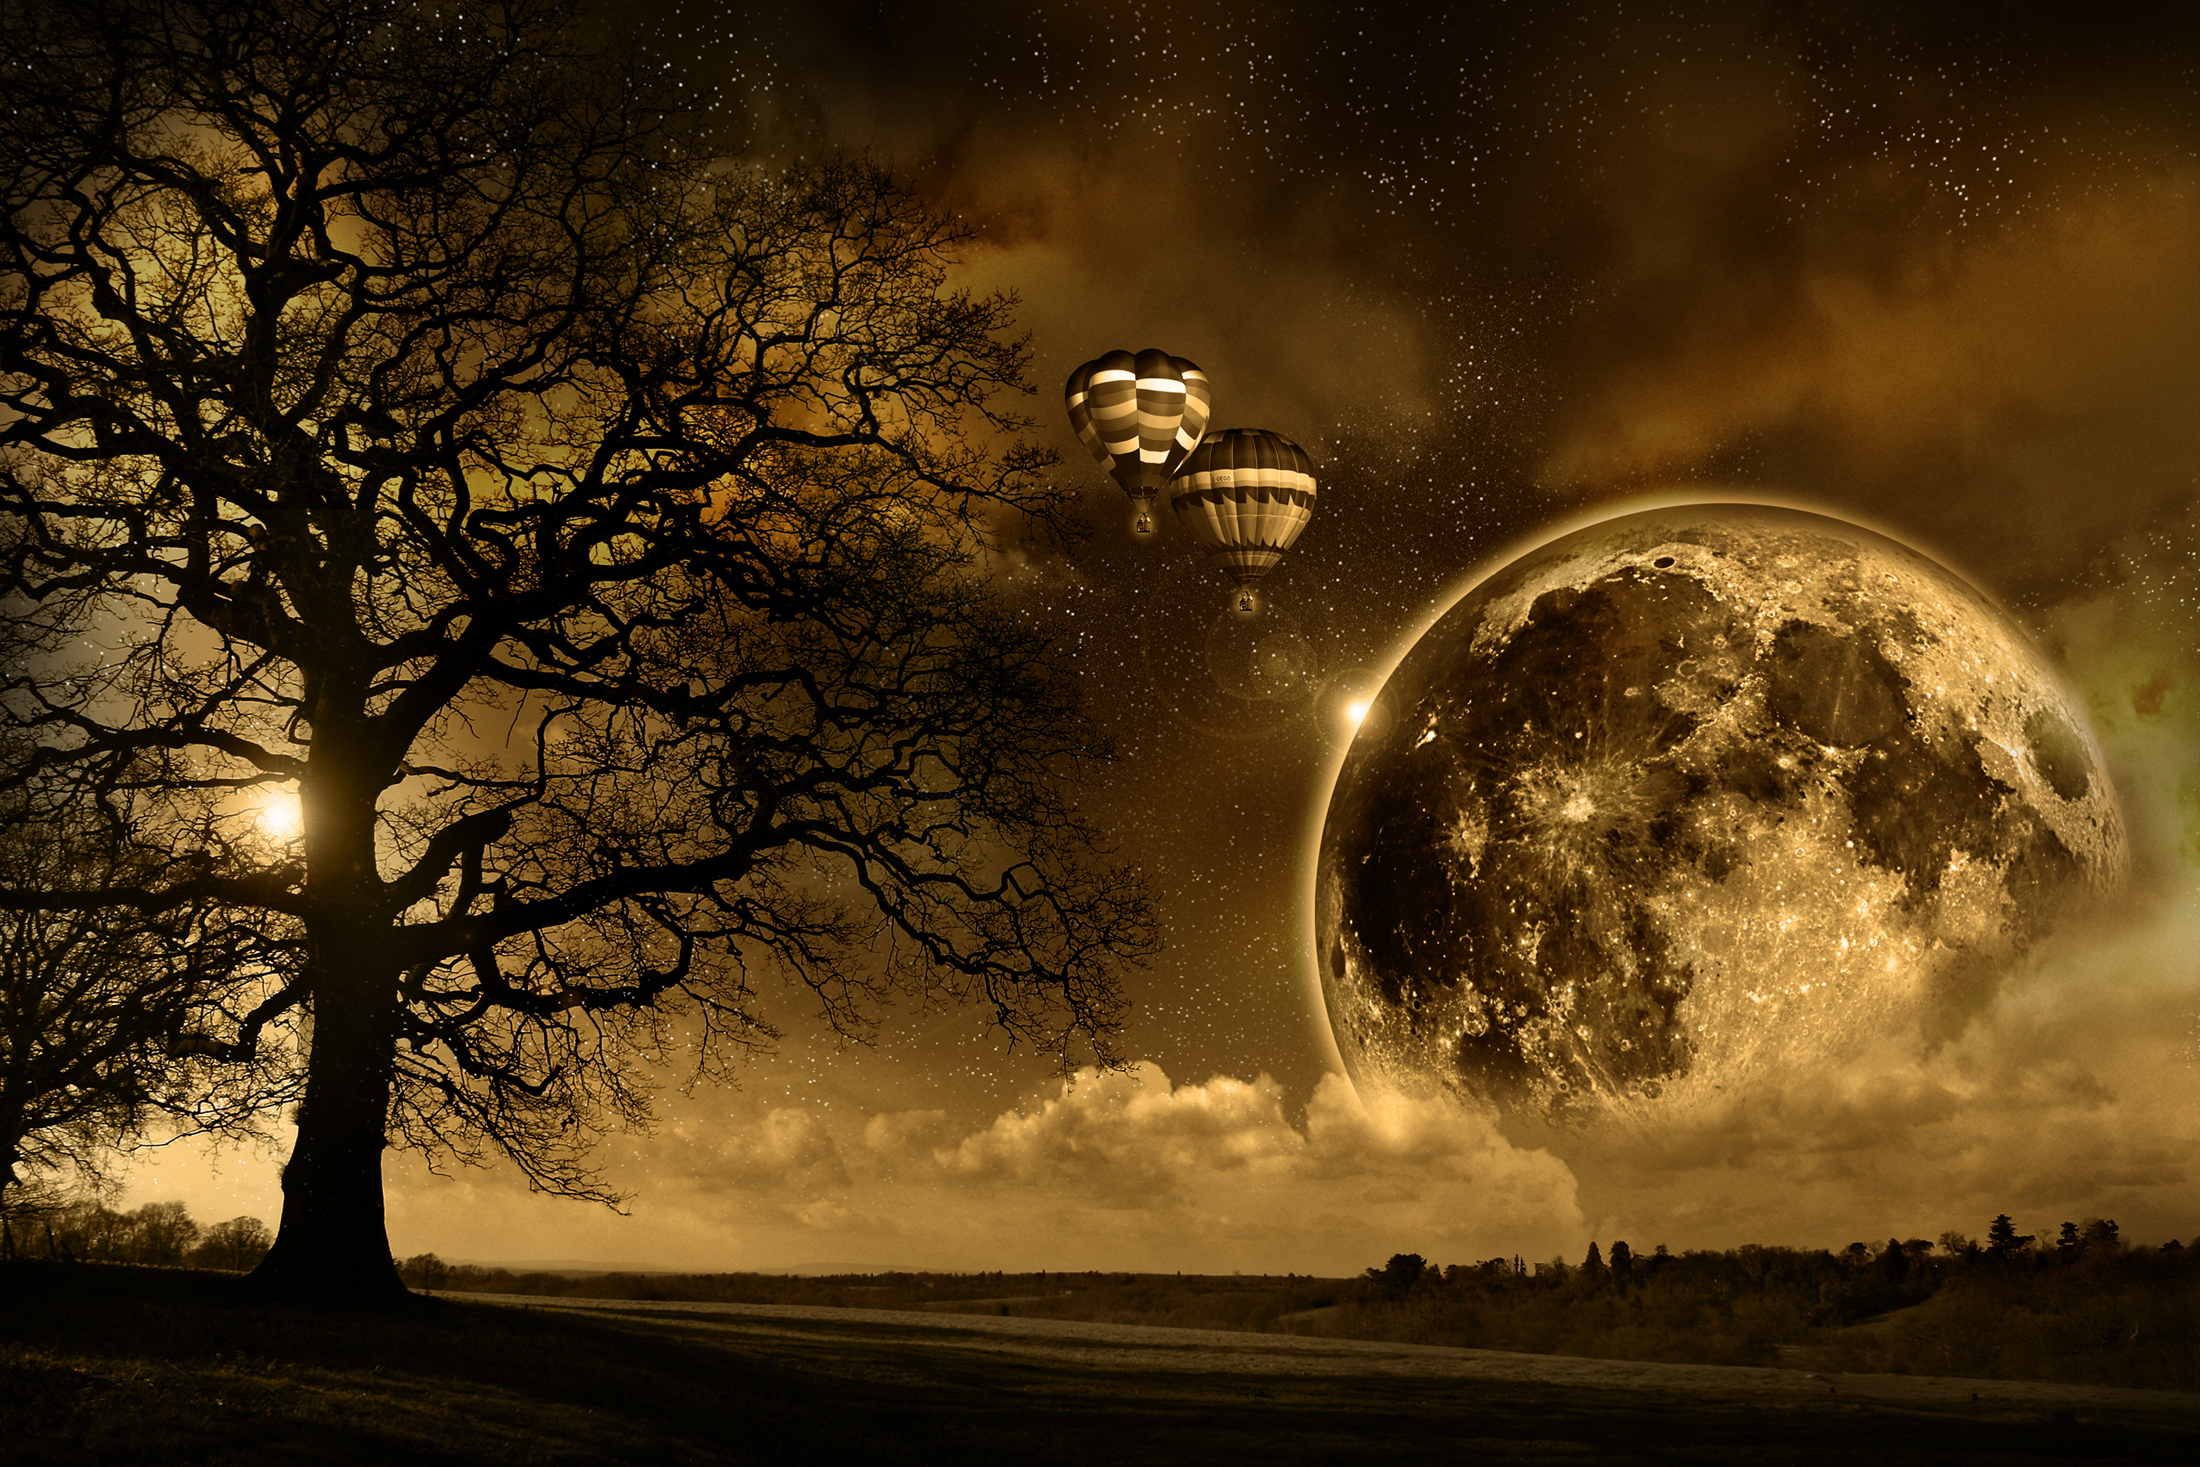
\includegraphics{images/index3.jpg}

Bem vindo! Este é um curso básico de ciências de dados para pessoas que estão começando.
Aqui você encontrará muita matemática, estatística, dados e referências à cultura pop.

\hypertarget{sobre-mim}{%
\section{Sobre mim}\label{sobre-mim}}

Eu decidi criar este curso para despertar o interesse de mais pessoas para a ciência de dados. Apesar de ser uma área já tão popular hoje em dia, seu conteúdo é denso, repleto de operações matemáticas, álgebra linear e estatística. Não se engane, vamos falar um pouco sobre estes temas aqui, mas espero conseguir trazê-los de uma forma leva e repleta de referências à cultura pop.

O objetivo deste curso não é formar novos cientistas de dados, mas apontá-los na direção certa. O conteúdo aqui presente não tem a intenção de ser o mais completo e detalhado, apenas de mostrar por exemplos como se desenvolve um projeto com dados, buscando dispertar o interesse de pessoas que possam não conhecer a área. Caso você já seja um cientista de dados, fica \sout{vai ter bolo}, quem sabe você aprende algo novo?

Eu me chamo Tiago Alves, sou mestre em Ciências da Computação pela UFMG desde 2018 e trabalho como
cientista de Dados desde 2016, já trabalhei com projetos nas áreas \ldots{} resolvendo problemas como \ldots{}

\url{http://tiagohca.com/}

\hypertarget{disclaimer}{%
\section{Disclaimer}\label{disclaimer}}

Este é um curso sob construção e em constante mudança. Eu sou responsável apenas pelo conteúdo escrito. Todos os direitos de imagens e propriedades intelectuais devems ser devidamente respeitados.

\hypertarget{um-buxe1sico-sobre-python}{%
\chapter{Um básico sobre python}\label{um-buxe1sico-sobre-python}}

Recomendo fortemente que você tenha alguma noção de programação, pelo menos o básico.

Se não tiver, vou tentar te explicar o necessário aqui.

Caso já saiba programar e já tenha utilizado Python, você pode pular para \protect\hyperlink{completando-o-pokedex---um-tutorial-sobre-como-obter-dados}{Completando o Pokedex - Um tutorial sobre como obter dados}

\hypertarget{configurando-o-ambiente}{%
\section{Configurando o ambiente}\label{configurando-o-ambiente}}

Antes de começar, precisamos instalar o Anaconda.

Acesse este \href{link}{https://www.anaconda.com/products/individual} e faça a instalação de acordo com o seu sistema.

Uma das melhores invenções do ser humano foi o Jupyter Notebook, vindo logo depois da internet e do microondas.

\hypertarget{o-primeiro-programa}{%
\section{O primeiro programa}\label{o-primeiro-programa}}

Programar é uma tarefa que envolver um forte raciocínio lógico. Não é algo complicado em sua essência, mas também não é algo que se aprenda em alguns minutos. Novamente, eu recomendo que você procure um curso especializado de programação caso esta seja sua primeira vez.

Aqui vou mostrar os primeiros passos para se começar a programar.

\hypertarget{bibliotecas-e-outras-ferramentas-uxfateis}{%
\section{Bibliotecas e outras ferramentas úteis}\label{bibliotecas-e-outras-ferramentas-uxfateis}}

Nos dias de hoje é raro construirmos programas do zero, graças às extensas comunidades existentes, independente da linguagem que você use. Python possui uma comunidade especialmente grande, com inúmeras bibliotecas públicas que agilizam muito o nosso trabalho. Lembre-se, não há por que reinventar a roda quando você pode comprar um carro.

\hypertarget{pandas}{%
\subsection{Pandas}\label{pandas}}

\hypertarget{scikit-learn}{%
\subsection{Scikit-Learn}\label{scikit-learn}}

\hypertarget{matplotlib}{%
\subsection{Matplotlib}\label{matplotlib}}

\hypertarget{plotly}{%
\subsection{Plotly}\label{plotly}}

\hypertarget{completando-o-pokedex---um-tutorial-sobre-como-obter-dados}{%
\chapter{Completando o Pokedex - Um tutorial sobre como obter dados}\label{completando-o-pokedex---um-tutorial-sobre-como-obter-dados}}

O primeiro passo de qualquer projeto de ciência de dados é\ldots{} conseguir os dados.

Para nossa sorte, existe uma tonelada de dados públicos que podem ser encontrados facilmente na internet. Algumas fontes boas de dados são \ldots{}

No nosso primeiro projeto vamos adentrar o mundo Pokémon! Para isto, precisamos de uma base de dados sobre os monstrinhos. A base que usaremos neste projeto pode ser encontrada \href{https://www.kaggle.com/rounakbanik/pokemon/data}{neste link} (você talvez tenha que criar uma conta). O Kaggle, plataforma onde está a base, é um excelente lugar para aprimorar seus conhecimentos em ciência de dados. Lá você encontra bases de dados, códigos e tutoriais feitos pela comunidade, fórums de discussão e competições emocionantes (algumas até chegam a pagar milhares de dólares para os vencedores!).

Assim como no mundo Pokémon encontramos diversas espécies quando entramos no mato alto, no mundo real encontramos diversos tipos de dados. Antes de mais nada vamos falar um pouco sobre estes tipos.

\hypertarget{tipos-de-dados}{%
\section{Tipos de dados}\label{tipos-de-dados}}

\hypertarget{tabular}{%
\subsection{Tabular}\label{tabular}}

\hypertarget{texto}{%
\subsection{Texto}\label{texto}}

\hypertarget{imagem}{%
\subsection{Imagem}\label{imagem}}

\hypertarget{uxe1udio}{%
\subsection{Áudio}\label{uxe1udio}}

\hypertarget{carregando-a-base-de-dados}{%
\section{Carregando a base de dados}\label{carregando-a-base-de-dados}}

\hypertarget{como-saber-tudo-o-que-huxe1-sobre-os-pokuxe9mon---a-anuxe1lise-exploratuxf3ria}{%
\chapter{Como saber tudo o que há sobre os Pokémon - A análise exploratória}\label{como-saber-tudo-o-que-huxe1-sobre-os-pokuxe9mon---a-anuxe1lise-exploratuxf3ria}}

Agora que já temos as informações sobre os monstrinhos precisamos descobrir o que elas estão nos dizendo. Esta é uma das partes mais cruciais do projeto, e quando executada com atenção pode te levar muito longe. O que vamos fazer chama-se E.D.A. (Exploratory Data Analysis, ou em português, Análise Exploratória dos Dados)

\hypertarget{descrevendo-os-pokuxe9mon---como-funciona-a-engenharia-de-features}{%
\chapter{Descrevendo os Pokémon - Como funciona a engenharia de features}\label{descrevendo-os-pokuxe9mon---como-funciona-a-engenharia-de-features}}

Agora que já entendemos bastante do dado, está na hora de começar a descrever os Pokémon de uma maneira que uma máquina entenda. Calma! Não vamos escrever zeros e ums! Mas precisamos de fato criar alguns números\ldots{}

A base de dados consiste de várias informações estruturadas sobre cada Pokémon e embora seja fácil para um ser humano interpretar o que está lá, a máquina pode ter dificuldade com algumas das colunas. Esta etapa chama-se Engenharia de Features (ou de Características). Uma feature nada mais é que uma caracterísica que ajuda a descrever alguma coisa. Por exemplo, nós seres humanos podemos ser descritos com apenas algumas features: idade, gênero, se assistiu todos os filmes do MCU ou não. O que vamos fazer agora é descrever os Pokémon como uma série de números onde cada um representa uma feature que iremos definir.

\hypertarget{one-hot-encoding}{%
\section{One-hot encoding}\label{one-hot-encoding}}

\hypertarget{label-encoding}{%
\section{Label encoding}\label{label-encoding}}

\hypertarget{normalizauxe7uxe3o}{%
\section{Normalização}\label{normalizauxe7uxe3o}}

\hypertarget{lenduxe1rio-ou-nuxe3o---um-primeiro-modelo-de-classificauxe7uxe3o}{%
\chapter{Lendário ou não? - Um primeiro modelo de classificação}\label{lenduxe1rio-ou-nuxe3o---um-primeiro-modelo-de-classificauxe7uxe3o}}

Quanto trabalho nos dados, não é mesmo? Não se preocupe, finalmente chegou a hora: vamos criar um modelo!

Um modelo é uma função \(y = f(x)\) \ldots{}

\bibliography{book.bib,packages.bib}

\end{document}
